\newcommand{\DocFooter}{DiGiTerra 0.1.0 verification record for the EDX deployment, 2026-09-25}
% Shared preamble for the three DiGiTerra audit documents. Compile with xelatex.
\documentclass[11pt,letterpaper]{article}
\usepackage[margin=1in]{geometry}
\usepackage{fontspec}
\setmainfont{Latin Modern Roman}
\setsansfont{Latin Modern Sans}
\setmonofont[Scale=0.9]{Latin Modern Mono}
\usepackage{microtype}
\usepackage{graphicx}
\graphicspath{{figures/}{figures/screens/}}
\usepackage{booktabs}
\usepackage{longtable}
\usepackage{array}
\usepackage{caption}
\captionsetup{font=small,labelfont=bf,justification=raggedright,singlelinecheck=false}
\usepackage{xcolor}
\usepackage[hidelinks]{hyperref}
\usepackage{enumitem}
\setlist{nosep}
\usepackage{parskip}
\setlength{\parskip}{6pt}
\usepackage{fancyhdr}
\pagestyle{fancy}
\fancyhf{}
\rfoot{\small\thepage}
\lfoot{\small\DocFooter}
\renewcommand{\headrulewidth}{0pt}
\newcolumntype{L}[1]{>{\raggedright\arraybackslash}p{#1}}
\usepackage{url}\usepackage{seqsplit}\DeclareRobustCommand{\code}[1]{\texttt{\seqsplit{#1}}}
\setlength{\emergencystretch}{2em}
\newcommand{\shot}[3]{\begin{figure}[htbp]\centering\includegraphics[width=#2\textwidth,height=0.42\textheight,keepaspectratio]{#1}\caption{#3}\end{figure}}
\setcounter{secnumdepth}{2}

\title{DiGiTerra 0.1.0: verification record, product comparison and deployment notes\\[4pt]\large Internal record for the NETL Energy Data eXchange deployment}
\author{Rowan R. Terra, Terra Cognita LLC and Duquesne University}
\date{25 September 2026}
\begin{document}
\maketitle

\paragraph{TL;DR.} The copy of DiGiTerra hosted on EDX is the same code as commit \code{5192687} on branch \code{audit-fixes}, and this record is what has been checked about it. The public release tag \code{v0.1.0} (2026-09-27) is later on that branch; the repository CHANGELOG lists what changed between the two. Ordinary least squares, k-nearest neighbors, logistic regression and descriptive statistics reproduce a scikit-learn script exactly and agree with R, Excel, Orange and AI Studio to better than $10^{-12}$ on every compared value except Orange's logistic probabilities on arm64 (up to $8\times10^{-3}$, cause inferred). The adversarial review of 2026-09-24 found 25 defects, three of them security findings in how a saved model was loaded, and 17 that changed a reported number; all are fixed and replayed by \code{scripts/adversarial\_check.py}, which is the pre-release gate. Against eleven alternatives, DiGiTerra's distinguishing rows are the run record (input hash, seed, package versions) and the signed artifact; its gaps are the blending rows (join, filter, formula columns, sampling), database sources and scripting. Every desktop alternative is free; the cloud alternatives bill by the hour and cannot run inside the laboratory network.

\tableofcontents

\section{Scope and records}

This document reports the verification work on DiGiTerra 0.1.0 as it stands at commit \code{5192687} on branch \code{audit-fixes} (tag \code{v0.1.0}), and places the application beside the no-code and low-code alternatives that a research group could use instead. Every number in the audit sections is read from a file in the repository, and the file is named beside the number. Every statement about another product is read from that product's own documentation or from the product itself running on one machine, and the source and the date are given.

Four records carry the audit. The differential test E1 (\code{docs/differential\_test\_E1/}) runs the same fixed train and test files through DiGiTerra and four independent programs and compares every printed value against a plain scikit-learn script. The adversarial review of 2026-09-24 (\code{CHANGELOG.md}, \code{tests/unit/test\_review\_2026\_09\_24.py}, \code{scripts/adversarial\_check.py}, \code{docs/adversarial\_check\_2026-09-25.json}) attacked the routes, the pipeline and the browser side and reproduced each defect before it was fixed. The estimator sweep (\code{docs/every\_model\_sweep\_2026-09-24.json}) trains every registered estimator through the function the web route calls. The artifact round trip (\code{docs/artifact\_roundtrip\_2026-09-24.json}) writes every fitted estimator to the bundle format, reads it back and compares predictions.

The comparison sections rest on two further records. The feature survey (\code{docs/competitor\_survey\_2026-09-24.txt}) reads eleven products' documentation on one day and tabulates steps to a first model, the novice and expert paths, hyperparameter access, data checks, the run record, accessibility claims, cost and deployment. The price survey (\code{docs/price\_survey\_2026-09-25.txt}) quotes each vendor's price page verbatim. Seven of the products were also installed and driven on one Apple silicon Mac on 2026-09-25 (Orange 3.39.0, Altair AI Studio 2026.0.1, KNIME Analytics Platform 5.12.0, Weka 3.8.7, JASP 0.98.1, jamovi 2.7.37 and Microsoft Excel 16.03), and H2O-3 3.46.0.7 with its Flow interface was started in a Linux container; the screenshots in Section~\ref{sec:interfaces} are from those sessions, not from vendor material.

Two limits apply throughout. The differential test covers ordinary least squares, k-nearest neighbors, multinomial logistic regression and descriptive statistics on two small public datasets; it says nothing about the other 64 estimators beyond what the sweep and the round trip say. The product comparison reads documentation and one installed copy of each product; a feature that a product carries but does not document, or carries in a paid tier that was not opened, is recorded as not stated rather than absent.


\section{Deployment context}
The National Energy Technology Laboratory hosts DiGiTerra on its internal Energy Data eXchange platform (EDX) as a laboratory-approved executable for staff who model geochemical and materials data without writing code. The Phase 2 application under which the application was accepted into the EDX Incubator (\code{docs/EDX\_Incubator\_Phase2\_Application\_Answers.pdf}) records the hosting terms, the initial user group with administrator and viewer roles, and the beta testers who held access to the repository before release. Two properties of the deployment bear on this record. The hosted copy and the public repository are one code base, so a run made inside the laboratory and a run made by an outside reviewer from the same commit carry the same manifest fields and can be compared line by line. And the hosted instance sits behind an institutional proxy that supplies the user identity, so the application implements no login of its own; the security findings in Section~\ref{sec:review} concern what a user can do with a file once inside, not the perimeter.

The cloud alternatives in Sections~\ref{sec:interfaces} to \ref{sec:prices} (SageMaker Canvas, Azure Machine Learning, Vertex AI, DataRobot SaaS) run only in the vendor's cloud and are therefore not candidates for data that stays inside the laboratory network; they are compared for what they show a non-programmer, not as deployment options.

\section{Differential test E1}
\label{sec:e1}

\subsection{Design}

E1 is a black-box differential test: the same inputs go into several programs written by different people, and the outputs are compared as printed. A plain scikit-learn 1.9.0 script (\code{scripts/oracle.py}) is the arbiter, so agreement with the arbiter is what the test measures; the arbiter itself is not assumed correct, and the three independent engines (R, Excel, AI Studio) are what give a disagreement its weight.

Two example datasets were shuffled once with a recorded permutation and split once into fixed train and test halves: the diabetes file into 353 and 89 rows, and the iris file into 120 and 30 rows. The split is written to disk (\code{data/}, with \code{md5sums.txt}) and every program reads the two halves as two tables; no program performs its own split, scaling, imputation, outlier handling, feature selection or hyperparameter search. A column named \code{order} carries the row identity and is excluded from the predictors everywhere.

Five cases were run. D1 and D2 are descriptive statistics of the two base files (n, mean, sample standard deviation, minimum, first quartile, median, third quartile, maximum; quartiles by the linear method that pandas, R type~7 and Excel \code{QUARTILE.INC} share). R1 is ordinary least squares on the diabetes training rows with ten predictors, compared on the intercept, the ten coefficients, the test RMSE, MAE and $R^2$, and all 89 test predictions. C1 is k-nearest neighbors on iris ($k=5$, Euclidean, uniform weights), compared on all 30 predicted classes. C2 is multinomial logistic regression on iris (L2, $C=1$, lbfgs, 100 iterations), compared on the 30 classes and the 90 class probabilities; R and AI Studio fit a differently regularized model and are excluded from C2 by plan, and Excel has no classifier.

DiGiTerra ran every case through its own routes (\code{/upload}, \code{/preprocess}, \code{/process}, \code{/export-bundle}, \code{/predict}) with the Advanced form's request, split method Time on the \code{order} column, test size 0.20, no scaler, seed 20260924 and ten decimal places. The other programs ran through their own interfaces: R 4.5.1 from a script, Orange 3.39.0 through its bundled Python, AI Studio 2026.0.1 from an imported process, Excel 16.03 from a workbook whose statistics and regression are Excel formulas (\code{COUNT}, \code{AVERAGE}, \code{STDEV.S}, \code{QUARTILE.INC}, \code{MEDIAN}, \code{LINEST}, \code{SUMXMY2}, \code{DEVSQ}).

\subsection{Controls}

Every program ran twice, with a close and reopen between runs, and the two saved outputs had to agree on every value. DiGiTerra ran R1 three times, twice at the start of the session and once at the end, and its predictions, coefficients and metrics files had to be byte-identical; only the run id, the timestamps and the artifact hash may differ. All controls passed for all five programs (\code{NOTEBOOK.txt}, entries marked CONTROLS PASS).

The comparison script (\code{scripts/compare.py}) formats every metric to \code{\%.6e} and classes each cell as \emph{same}, \emph{last digit} (mantissa differs by one unit in the last place), \emph{near zero} (both values within $10^{-12}$ of zero, which is where the centered diabetes columns land), \emph{rounded} (the value equals the arbiter rounded to a stated number of decimals), \emph{within $10^{-6}$}, or \emph{other}. The pass rule for a same-engine program (Orange, which runs scikit-learn) is zero \emph{other} cells and zero class mismatches; for an independent engine it is a relative difference below $10^{-6}$ on every value.

\subsection{Results}

Figure~\ref{fig:e1} counts every compared cell by program, case and class, from \code{RESULTS.csv} (2,436 cells after the 2026-09-25 completion). Figure~\ref{fig:e1r1} shows the relative differences behind the R1 bars, and Figure~\ref{fig:orange} the one set of cells classed \emph{other}.

\begin{figure}[htbp]
\centering
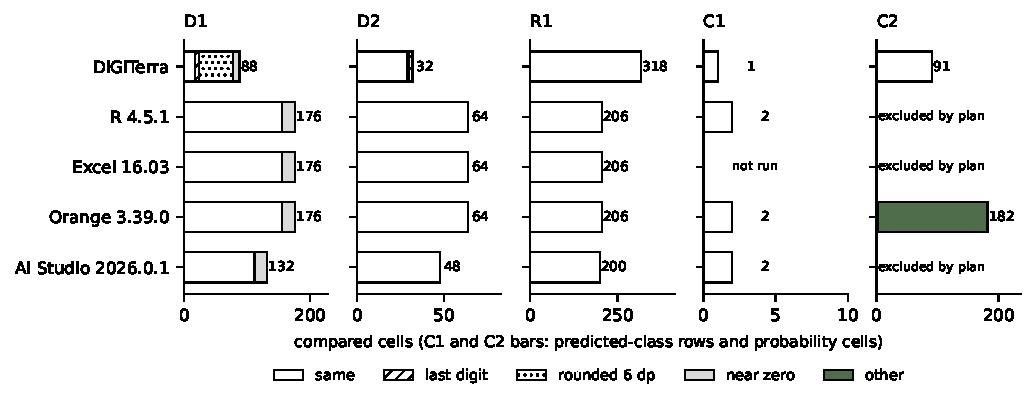
\includegraphics[width=\textwidth]{fig_e1_agreement}
\caption{E1 agreement by program and case. Each bar counts the compared cells; the fill marks the class. DiGiTerra's D1 and D2 bars carry \emph{rounded 6 dp} and \emph{last digit} cells because the application prints descriptive statistics to six decimals (a change made during the test; the original rounding was four). \emph{Near zero} cells are the ten centered diabetes means, which every program prints as a value within $10^{-16}$ of zero. Source: \code{docs/differential\_test\_E1/RESULTS.csv}.}
\label{fig:e1}
\end{figure}

\begin{figure}[htbp]
\centering
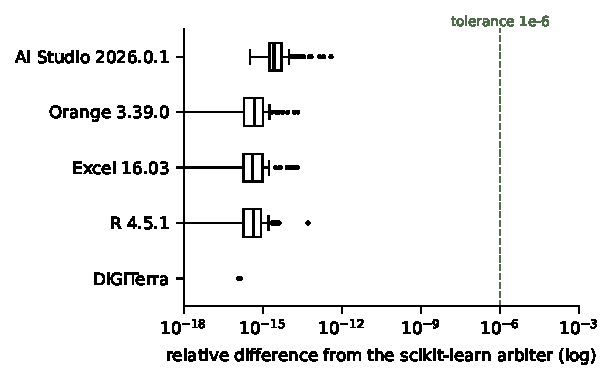
\includegraphics[width=0.6\textwidth]{fig_e1_r1_reldiff}
\caption{R1 ordinary least squares: relative difference from the arbiter for the intercept, the ten coefficients and the 89 test predictions, by program. DiGiTerra's cells are zero except three predictions at $1.4\times10^{-16}$ (one unit in the last place of the printed value); zeros are drawn at the axis floor. Every independent engine agrees with the arbiter to better than $10^{-12}$, six orders inside the $10^{-6}$ tolerance. Source: \code{RESULTS.csv}, case R1.}
\label{fig:e1r1}
\end{figure}

\begin{figure}[htbp]
\centering
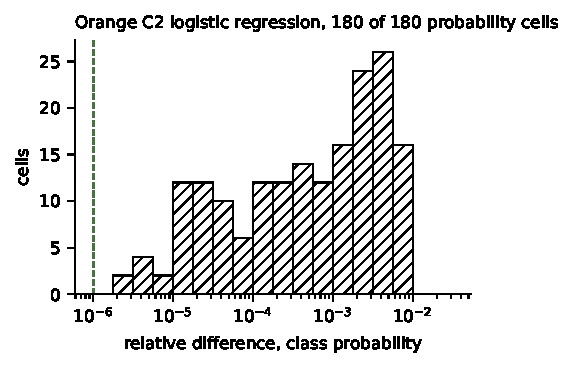
\includegraphics[width=0.6\textwidth]{fig_e1_orange_c2}
\caption{Orange C2: relative difference of the 90 class probabilities from the arbiter (180 cells over two runs). All 30 predicted classes agree; the probabilities differ by up to $7.9\times10^{-3}$. Source: \code{RESULTS.csv}, app orange, case C2.}
\label{fig:orange}
\end{figure}

R1 is the strongest result. The intercept, the ten coefficients and all 89 test predictions agree across DiGiTerra, R, Excel, Orange and the arbiter at six significant figures, and the largest relative difference on any R1 cell among the four reference programs is $3.8\times10^{-13}$ (AI Studio); R, Excel and Orange stay below $6\times10^{-14}$. DiGiTerra's own metrics differ from the arbiter by at most $3.6\times10^{-11}$ ($R^2$, printed to ten decimals). AI Studio agrees on the ten coefficients and the 89 predictions; its export omits the intercept, and its \code{squared\_correlation} is the squared Pearson correlation (0.5201965) rather than $R^2$ (0.5195044), which the plan anticipated, so $R^2$ was recomputed from AI Studio's own predictions and matches. C1 agrees on all 30 classes in every program that ran it. C2 agrees on all 30 classes in Orange, and DiGiTerra reproduces the arbiter's 90 probabilities exactly.

The Orange probability gap is the one open cell. Orange 3.39.0 bundles scikit-learn 1.5.2 on arm64. The same library version on x86\_64 gives the arbiter's probabilities (0.97462567 for the first row, not Orange's 0.97454283), a one-versus-rest fit gives 0.87, and a tight fit (tolerance $10^{-10}$, 116 iterations) differs from both. The remaining variable is the platform arithmetic under the loose default tolerance (arm64 Accelerate against x86\_64 OpenBLAS). That attribution is inferred, not established; it becomes established when \code{scripts/oracle.py} is run under Orange's own Python on the Mac and reproduces Orange's numbers. The \code{NOTEBOOK.txt} entry of 2026-09-24T17:40Z records the state.

Excel and AI Studio descriptive statistics were added on 2026-09-25 and completed the set. Excel's D1 and D2 agree on every one of the eight statistics for every column (156 cells same and 20 near zero for D1; 64 same for D2), and its R1 matches on 206 cells. AI Studio's Aggregate operator has no quartile function, so its D1 and D2 carry six statistics rather than eight (112 same and 20 near zero; 48 same). With those in place the comparison script reports the set as COMPLETE (\code{RESULT\_2026-09-25.txt}).

\subsection{What the test found in DiGiTerra}

Three defects were established in the version under test (tree \code{0942e0c}) and corrected before the results above were produced; the pre-fix outputs are kept in \code{digiterra\_outputs\_pre\_fix\_0942e0c/}. First, the regression metrics on the page and in the manifest were rounded to three decimals before the decimal-places setting was applied, so a setting of ten printed \code{53.8080000000} for a test RMSE of 53.808429803715498. Second, descriptive statistics were rounded to four decimals, so the diabetes means printed as $-0.0$. Third, for nineteen classifiers a hyperparameter typed on the Advanced form never reached the estimator while the run record still recorded the request; KNeighbors with \code{n\_neighbors} 3 was fitted with 5. The first two are closed by \code{tests/unit/test\_decimal\_setting.py} and the E1 rerun; the third by \code{test\_knn\_classifier\_form\_values\_reach\_the\_estimator} and the pass-through of form values for all nineteen. The third finding is the one a user could not have seen: the manifest said 3 and the model used 5.

\section{Adversarial review of 2026-09-24}
\label{sec:review}

Three reviewers worked in parallel, one each on the HTTP routes, the modeling pipeline and the browser side, with the instruction to break the application rather than to describe it. Each reviewer had to reproduce a defect before it counted; the reproduction is what became the regression test. The review reported 25 reproduced defects. The changelog records them in fourteen entries, several of which bundle more than one fault; Table~\ref{tab:defects} separates the entries into the faults a reader would want to test one by one, which gives 29 rows. The count in the changelog is the reviewers'; the itemization is this document's.

\small\begin{longtable}{@{}L{0.5cm}L{1.6cm}L{7.6cm}L{1.6cm}L{3.4cm}@{}}
\caption{Defects reproduced by the review, by area. \emph{Effect} says what a user would have seen: a wrong number (result), code execution from a file (security), a run that failed or silently ignored an input (behavior). Every row is fixed at \code{5192687}; the test column names the file that guards it.}\label{tab:defects}\\
\toprule
\# & Area & Defect as reproduced & Effect & Guard \\
\midrule
\endfirsthead
\toprule
\# & Area & Defect as reproduced & Effect & Guard \\
\midrule
\endhead
1 & routes & The artifact type allowlist was a prefix test, so \code{builtins.eval} matched \code{builtins}. & security & \code{test\_bundle.py}, crafted artifact \\
2 & routes & The loader handed skops the file's own type list as trusted, so a crafted \code{model.skops} ran code on load. & security & same \\
3 & routes & The disk session store carried no signature on its objects file. & security & \code{test\_bundle.py} \\
4 & routes & Two workbook routes returned raw exception text to the client. & behavior & \code{adversarial\_check.py} \\
5 & routes & A spreadsheet cell starting with \code{=}, \code{+}, \code{-} or \code{@} was written as a formula. & security & \code{adversarial\_check.py} \\
6 & pipeline & A model with no editable table sent no hyperparameters and \code{get\_model\_kwargs} passed \code{None} values to the trainer; the guided page's default run failed for 14 models. & behavior & \code{test\_review\_2026\_09\_24.py} \\
7 & pipeline & Mean, median and mode fills included the target column, so a made-up target was trained on and scored as truth. & result & same \\
8 & pipeline & Binary ROC AUC scored the string labels against the second probability column and inverted the AUC whenever the string order differed from the class order. & result & same \\
9 & pipeline & Average precision failed on string labels and was silently omitted. & result & same \\
10 & pipeline & IQR and z-score outlier removal read the one-hot columns and deleted every training row of a category under 25 percent. & result & same \\
11 & pipeline & With feature selection on, the novelty score was never written at prediction time. & behavior & same \\
12 & pipeline & Cross-validation did not apply a deferred mean or median fill, so an estimator that refuses NaN failed after the model had trained. & behavior & same \\
13 & pipeline & Cross-validation scored only the first of several targets. & result & same \\
14 & pipeline & Cross-validation ignored a grouped or time-ordered split plan in favor of shuffled folds (a grouped holdout of $R^2$ $-2.2$ came with a CV of 0.95). & result & same \\
15 & pipeline & Seed 0 was replaced by a random seed. & result & same \\
16 & pipeline & GaussianMixture never received the seed. & result & same \\
17 & pipeline & GradientBoosting \code{warm\_start} was inverted. & result & same \\
18 & pipeline & Fill with the mode did nothing and the rows were dropped. & result & same \\
19 & pipeline & Remove rows with zeros removed only rows that were zero in every scoped column. & result & same \\
20 & pipeline & A numeric column chosen for one-hot encoding was listed twice and raised a duplicate-column error. & behavior & same \\
21 & pipeline & The AutoML page said a blank model would be chosen by AutoML and sent a random forest. & result & same \\
22 & browser & Hyperparameters whose scikit-learn default is \code{None} were sent as strings (\code{max\_depth: "3"}). & result & guided browser suite \\
23 & browser & Integer fields truncated 2.5 to 2 and 0.5 to 0. & result & same \\
24 & browser & Stratifying by the target was silently dropped. & result & same \\
25 & browser & Two quick model changes could leave the first model's hyperparameter table under the second. & result & same \\
26 & browser & A cleared seed, decimal-places or folds field was sent as 0. & result & same \\
27 & browser & Escape did not close a tooltip opened by keyboard focus. & behavior & same \\
28 & browser & A failed model list or a dead progress stream left the page without a message. & behavior & same \\
29 & browser & A failed column read after a good upload was reported as an upload failure. & behavior & same \\
\bottomrule
\end{longtable}\normalsize

Seventeen rows change a number a reader would have trusted. Three of them deserve a sentence each because a manifest would not have revealed them. Row 7 let a fill step write the training mean into blank target cells, so the model learned and was scored on values that were never observed; the manifest recorded the fill as requested and gave no sign that the target was in scope. Row 8 turned a good binary classifier into a bad one on paper whenever the positive class sorted first alphabetically; every other metric on the page was right, so the inverted AUC stood beside a correct accuracy. Row 14 reported a cross-validation score from shuffled folds beside a holdout that honored the grouped or time-ordered plan, so the two numbers described different experiments while sharing one results page.

Rows 1 to 3 are the security findings. A bundle is signed with an installation key and verified on import, but a prefix test on the type allowlist admitted a builtin, and the loader trusted the type list inside the file rather than the application's own. The allowlist is now an exact set written by a census of every registered estimator (\code{python\_scripts/reporting/artifact\_allowlist.txt}, 66 of 67 estimators write and load; \code{birch} is refused rather than loaded unsafely), skops is given that list and never the file's, and the disk session store signs its objects file at save and verifies it at load with the same key.

Every probe the three reviewers ran is preserved as \code{scripts/adversarial\_check.py}. It replays the route attacks, the pipeline tests and the browser attack with a hostile CSV whose headers and labels carry markup, and prints PASS or FAIL per probe with what it saw. On \code{5d480a3} it printed 10 of 10 in the container with the pinned Chromium (\code{docs/adversarial\_check\_2026-09-25.json}); the record from the day of the review is \code{docs/adversarial\_check\_2026-09-24.json}. It runs in about six minutes and is the check to run before any release.

\section{Estimator sweep and artifact round trip}
\label{sec:sweep}

The registry names 69 entries: 33 regression, 24 classification and 12 clustering. The sweep (\code{scripts/every\_model\_sweep.py}, record \code{docs/every\_model\_sweep\_2026-09-24.json}) trains each entry on a matching example dataset through the same function the web route calls, with the hyperparameters an empty form submits, so it exercises the path a user takes rather than a test harness of its own. Sixty-seven entries train; \code{Polynomial} (regression) and \code{Perceptron} (classification) are registered without a train function and are skipped, which is the state the registry is in rather than a failure of the two estimators. The whole sweep takes 49 minutes on the container's two cores; four estimators account for most of it (Figure~\ref{fig:seconds}): SVM regression at 385 seconds, RadiusNeighbors at 348, NuSVR at 291 and HistGradientBoosting at 240, all on the 442-row diabetes file with default settings and no search.

\begin{figure}[htbp]
\centering
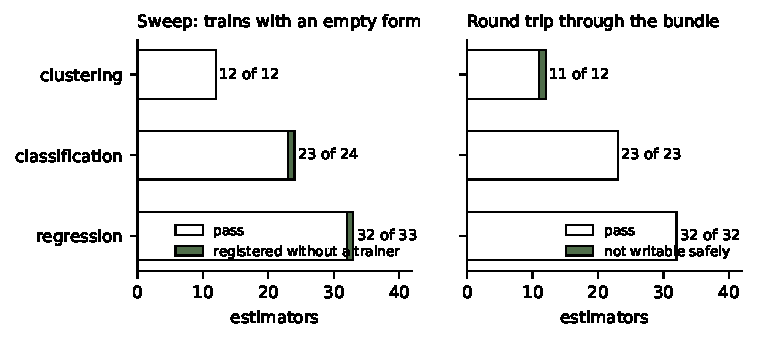
\includegraphics[width=0.75\textwidth]{fig_sweep_roundtrip}
\caption{Left: estimators that train with an empty form, by task. Right: estimators whose predictions are identical after a write to the bundle format and a read back. Sources: \code{every\_model\_sweep\_2026-09-24.json}, \code{artifact\_roundtrip\_2026-09-24.json}.}
\label{fig:sweep}
\end{figure}

\begin{figure}[htbp]
\centering
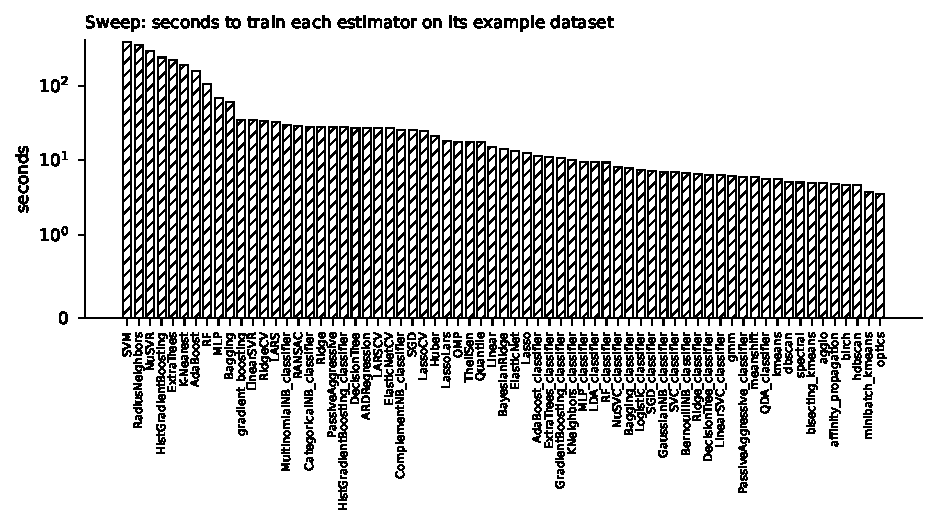
\includegraphics[width=\textwidth]{fig_sweep_seconds}
\caption{Seconds to train each of the 67 estimators in the sweep, symmetric log scale. Source: \code{every\_model\_sweep\_2026-09-24.json}.}
\label{fig:seconds}
\end{figure}

The round trip (\code{scripts/check\_artifact\_roundtrip.py}, record \code{docs/artifact\_roundtrip\_2026-09-24.json}) takes each of the 67 fitted estimators, writes it with skops 0.14.0 under the exact type allowlist, reads it back, and compares the predictions for the first eight rows of the dataset exactly, not within a tolerance. Sixty-six round-trip identically. \code{birch} cannot be written under the allowlist, and the application says so at export rather than writing an artifact that would need an unlisted type to load. The record stores the dataset hash, the seed, the artifact hash and both prediction vectors for every row, so a reader can rerun one estimator with \code{--only <model>} and compare against the stored numbers.

Together the two records bound the claim the paper makes about the registry. The application can train 67 estimators from its own form and can write and reload 66 of them; it does not claim that every hyperparameter of every estimator has been exercised, and the E1 finding on the nineteen classifiers (Section~\ref{sec:e1}) is the reason that claim is not made.

\section{The interfaces, side by side}
\label{sec:interfaces}

Every screenshot in this section was taken from the product running on the same Mac on 2026-09-25 (DiGiTerra and H2O Flow in a Linux container on the same day), at the point where a user has data loaded and is about to choose or configure a model. Where a product offers more than one path to a model, the screenshot shows the path its own welcome screen or documentation puts first. The comparison rests on four measurable properties rather than on a judgment of taste: how many separate screens or objects a user must create before a model is fitted; whether the model's settings are visible on the screen where the model is chosen; whether the interface can be used without composing a graph or writing a command; and whether a machine-readable record of the run is written without a further action.

\subsection{DiGiTerra}

\shot{shot_digiterra_guided_step3_full}{0.95}{DiGiTerra guided page, step 3 of 4, Full mode, after \code{iris.csv} was uploaded and \code{species} chosen as the target. The task, the model, the hyperparameter table with scikit-learn's defaults, the split, the scaler, feature selection, outlier handling, cross-validation and search are on one screen; each control carries a help button whose text is the explanation the screen reader gets. Guided mode hides everything below the model select.}

\shot{shot_digiterra_guided_step4}{0.95}{DiGiTerra guided page, step 4, after the run: the figures first, then the metrics against the baseline, then the downloads (predictions, manifest, model card, bundle).}

The guided page holds four steps, each filling the window with no scrolling: upload, target, model and run, result. A model is fitted after three steps (upload, choose the target, fit), with the fourth step showing the result. In Full mode the hyperparameter table is filled from the estimator's own signature through a route, so the names and defaults cannot drift from scikit-learn; a blank cell keeps the default. The manifest, model card and bundle are written by the run itself, and the manifest carries the SHA-256 of the uploaded bytes, the seed, the request as submitted, the fitted parameters, the split, the metrics, the baseline, the data-check findings and the version of every installed package.

\subsection{Node-graph tools: Orange, KNIME, AI Studio}

\shot{shot_orange_workflow}{0.95}{Orange 3.39.0, the Classification Tree example workflow from its own welcome screen. A model exists once a File widget, a learner widget and a viewer widget are placed and wired; the learner's settings are in a separate dialog opened by double-clicking the widget.}

\shot{shot_orange_tree_dialog}{0.95}{Orange, the Classification Tree widget's settings dialog opened over the workflow. Five parameters are exposed; the learner has more in scikit-learn, and the widget passes fixed values for the rest.}

\shot{shot_knime_workflow}{0.95}{KNIME Analytics Platform 5.12.0, the ``Combine Clean and Summarize Spreadsheet Data'' example from its welcome screen (no learner is in this example; the modeling nodes follow the same pattern). Each node opens its own configuration dialog; execution state is the traffic light under the node.}

\shot{shot_aistudio_design}{0.95}{Altair AI Studio 2026.0.1, Design view, with the E1 statistics process loaded and the Aggregate operator selected. The parameters of the selected operator appear in the right pane; the operator tree on the left lists the catalogue (Data Access 62, Blending 81, Cleansing 28, Modeling 167, Scoring 13, Validation 30, Utility 85 operators in this installation).}

\shot{shot_aistudio_automodel}{0.95}{AI Studio, the Auto Model wizard: six screens (Load Data, Select Task, Prepare Target, Select Inputs, Model Types, Results). Its output can be opened as a process in the Design view, which is the novice-to-expert path the feature survey recorded.}

In the three node-graph tools a model is the result of a graph: the user places a reader, a learner and an applier or evaluator, wires them, and runs the graph. The settings of any one node are in a dialog or pane that belongs to that node, so the model's hyperparameters and the split are never on the same screen unless the user arranges the panes so. Orange's example reaches a fitted tree with three widgets and two connections; the KNIME example carries about ten nodes; the E1 statistics process in AI Studio needed three operators per dataset. AI Studio's Auto Model wizard is the exception that proves the pattern: it walks a novice through six screens without a graph, then hands over a graph to edit. Orange writes a report file on request and KNIME keeps a log; AI Studio saves the process. None of the three documents a hash of the input or the installed package versions in that record (survey column ``Run record'').

\subsection{Notebook cells: H2O Flow}

\shot{shot_h2o_flow_model_menu}{0.95}{H2O Flow (H2O-3 3.46.0.7), the Assistance list that a new flow opens with. Every action is a routine name (\code{importFiles}, \code{buildModel}, \code{predict}) that runs in a cell; the cell above shows the command \code{assist}.}

\shot{shot_h2o_flow_glm_form}{0.95}{H2O Flow, the Build a Model form for a generalized linear model, scrolled to the regularization settings. Each field carries its description at the right; the form is long enough to need several screens of scrolling, and the frame, the response column and the model type are chosen higher on the same form.}

Flow is a notebook. A user clicks a routine in the Assistance list or types its name in a cell, runs the cell, and reads the output below it; building a model opens a form inside a cell whose length depends on the algorithm (the GLM form runs to several screens). The frame must be imported and parsed in earlier cells before the form can name it. The notebook is the run record, and a seed field is on the form. H2O's documentation marks Flow as deprecated (Section~\ref{sec:sources}, H2O), so the interface is compared here as the current no-code path to H2O-3 rather than as a maintained product.

\subsection{Form-driven statistics packages: JASP and jamovi}

\shot{shot_jasp_knn_form}{0.95}{JASP 0.98.1, k-nearest neighbors classification from the Machine Learning module, with the telco churn example loaded. The analysis is a form beside the data; the results table on the right fills as soon as a target and features are dropped in. The module lists nine regression, nine classification and five clustering methods.}

\shot{shot_jamovi_regression}{0.95}{jamovi 2.7.37, Linear Regression with Anderson's iris data. The analysis panel and the results panel share the window; jamovi's own machine learning module is a separate install from its library.}

JASP and jamovi are the closest in shape to DiGiTerra's guided page: a form beside the data, with results that update as the form changes, and no graph. Both are built for classical statistics, and their machine learning is a module: JASP ships one with 23 methods; jamovi's arrives from its module library. Both expose model settings in collapsible sections of the same form. Neither writes a run record beyond its own file format (\code{.jasp}, \code{.omv}), and neither documents a hash of the input or the package versions. JASP's own accessibility statement says screen readers are not supported; jamovi's says the interface can be operated from the keyboard and works with NVDA and JAWS (Section~\ref{sec:sources}).

\subsection{Dialog trees: Weka Explorer}

\shot{shot_weka_explorer_classify}{0.95}{Weka 3.8.7 Explorer, Classify tab, with \code{iris.arff} loaded. The classifier is chosen from a tree of package names; the test options and the class column are on the same tab.}

\shot{shot_weka_object_editor}{0.95}{Weka, the GenericObjectEditor dialog for the chosen classifier. Every option of the Java class is a field; the field names are the Java property names.}

Weka's Explorer is four tabs and two dialogs to a model: open a file, switch to Classify, choose a classifier from a package tree, edit its options in the object editor, start. Every option of the estimator is reachable, named as in the Java source. The run information in the output pane records the seed and the options; there is no file-level record without a further action.

\subsection{Spreadsheet: Excel}

\shot{shot_excel_r1_linest}{0.95}{Microsoft Excel 16.03, the E1 workbook's R1 sheet: the intercept and coefficients from \code{INDEX(LINEST(\ldots))}, the coefficient row, and the 89 test predictions from \code{SUMPRODUCT}. Excel is in E1 as a reference engine, not as a machine learning interface.}

Excel is in this comparison because it is the tool a research group already has and because its \code{LINEST} agreed with the arbiter on every R1 value (Figure~\ref{fig:e1r1}). It has no classifier, no split, no cross-validation and no run record; the workbook is the record, and the formulas are visible in it.

\subsection{Steps to a first model}

Table~\ref{tab:steps} restates the survey's count of steps to a first model for every product, with the installed products checked against the screens above. A step is a separate screen, dialog, widget or cell that the user must open or create; a click that changes a value on a screen already open is not a step.

\begin{table}[htbp]
\caption{Steps to a first fitted model, and where the model's settings are. From \code{docs/competitor\_survey\_2026-09-24.txt}, checked against the installed products on 2026-09-25 where a copy was available.}
\label{tab:steps}
\small
\begin{tabular}{@{}L{4.0cm}L{2.6cm}L{4.4cm}L{4.0cm}@{}}
\toprule
Product & Steps & Settings shown & Run record without a further action \\
\midrule
DiGiTerra guided page & 3 (upload, target, fit) & On the model step, one screen & Manifest, model card, bundle \\
Orange 3 & About 4 (3 widgets, wiring) & Widget dialog, per widget & Report on request \\
KNIME Analytics Platform & About 5 to 6 (3 to 5 nodes) & Node dialog, per node & \code{knime.log}, Hub versions \\
AI Studio, Auto Model & 6 wizard screens & Model Types screen & Saved process \\
AI Studio, Design & 3 operators and wiring & Parameters pane of the selected operator & Saved process \\
H2O-3 Flow & About 5 cells & Build Model form in a cell & The flow notebook \\
SageMaker Canvas & About 5 to 6 screens & Metric, algorithms, split only & Model versions, leaderboard \\
Azure Machine Learning AutoML & About 6 screens & Not per model in the UI & Jobs and child jobs \\
Vertex AI AutoML tabular & Not retrievable & Not stated & Not stated \\
Weka Explorer & 4 (2 tabs, 2 dialogs) & Object editor dialog & Run information in the output pane \\
JASP & About 4 & On the analysis form & \code{.jasp} file \\
jamovi & About 5 with a module & On the analysis form & \code{.omv} file \\
DataRobot & About 4 screens & Advanced Tuning & Seed, compliance DOCX \\
\bottomrule
\end{tabular}
\end{table}

\section{Capability coverage against the operator catalogues}
\label{sec:coverage}

AI Studio's operator reference is the most complete published catalogue among the products compared, so it is the yardstick here: every operator group in \code{docs.rapidminer.com/latest/studio/operators/} (read 2026-09-25) is mapped to what DiGiTerra 0.1.0 offers, and the other products are placed on the same rows from their documentation and the installed copies. Table~\ref{tab:coverage} is the map. \emph{Yes} means the capability is on the form or in the pipeline; \emph{part} means a subset; \emph{no} means absent; \emph{n/a} means the row does not apply to the product's purpose. The DiGiTerra column is read from the code; the other columns are read from documentation and one installed copy, so a \emph{no} there means not found on the pages and screens consulted, and a reader who knows a product better should treat such a cell as a claim to check rather than a verdict.

{\small\setlength{\tabcolsep}{3pt}\begin{longtable}{@{}L{2.4cm}L{3.9cm}L{1.35cm}L{1.35cm}L{1.05cm}L{1.05cm}L{1.35cm}L{1.05cm}L{1.35cm}@{}}
\caption{Capability rows from the AI Studio operator groups, with DiGiTerra and six other products. Columns: DiGiTerra (DG), AI Studio (AIS), Orange (Or), KNIME (KN), H2O Flow (H2O), JASP (JA), Weka (We). Sources: operator reference, product documentation and the installed copies of 2026-09-25; DiGiTerra from its guided page (\code{templates/guided.html}) and pipeline modules.}\label{tab:coverage}\\
\toprule
Group & Capability & DG & AIS & Or & KN & H2O & JA & We \\
\midrule
\endfirsthead
\toprule
Group & Capability & DG & AIS & Or & KN & H2O & JA & We \\
\midrule
\endhead
Data access & Read CSV, Excel, Parquet & yes & yes & part & yes & part & part & part \\
Data access & Read from a database or cloud store & no & yes & yes & yes & yes & yes & yes \\
Data access & Repository or project store & no & yes & no & yes & no & no & no \\
Blending, attributes & Select and rename columns & part & yes & yes & yes & yes & yes & yes \\
Blending, attributes & Type conversion (nominal, numeric, date) & no & yes & yes & yes & part & part & part \\
Blending, attributes & One-hot encoding & yes & yes & yes & yes & auto & no & yes \\
Blending, attributes & Target encoding & no & yes & no & yes & yes & no & no \\
Blending, attributes & Generate attributes by formula & no & yes & yes & yes & no & yes & yes \\
Blending, attributes & Remove correlated or useless columns & part (data checks) & yes & no & yes & no & no & yes \\
Blending, examples & Filter rows by condition & no & yes & yes & yes & no & yes & yes \\
Blending, examples & Sampling (random, stratified, bootstrap) & no & yes & yes & yes & no & no & yes \\
Blending, examples & Split data (random, stratified, time, group) & yes & part & yes & yes & part & part & part \\
Blending, table & Join, append, pivot & no & yes & yes & yes & yes & no & no \\
Cleansing & Missing values (mean, median, mode, drop) & yes & yes & yes & yes & auto & no & yes \\
Cleansing & Normalize or scale (standard, min-max, robust, quantile) & yes & yes & yes & yes & part & no & yes \\
Cleansing & Binning or discretization & no & yes & yes & yes & no & no & yes \\
Cleansing & Duplicates & part (check) & yes & yes & yes & no & no & yes \\
Cleansing & Outliers (IQR, z-score, isolation forest, LOF) & yes & yes (COF, LOF, distance, density) & yes & yes & no & no & yes \\
Cleansing & PCA, ICA, SVD & no & yes & yes & yes & yes & yes & yes \\
Modeling, predictive & Trees, forests, boosting & yes & yes & yes & yes & yes & yes & yes \\
Modeling, predictive & Linear, ridge, lasso, elastic net & yes & part & yes & yes & yes & yes & yes \\
Modeling, predictive & Logistic regression & yes & yes & yes & yes & yes & yes & yes \\
Modeling, predictive & SVM & yes & yes & yes & yes & yes (PSVM) & yes & yes \\
Modeling, predictive & Naive Bayes & yes & yes & yes & yes & yes & yes & yes \\
Modeling, predictive & k-NN & yes & yes & yes & yes & no & yes & yes \\
Modeling, predictive & Neural network (MLP) & yes & yes & yes & yes & yes & yes & yes \\
Modeling, predictive & Discriminant analysis & yes & yes & no & yes & no & yes & yes \\
Modeling, predictive & Rule induction & no & yes & yes & yes & yes (RuleFit) & no & yes \\
Modeling, predictive & Gaussian process, Bayesian ridge, robust regressors & yes & part & no & part & no & no & part \\
Modeling, predictive & Ensembles (bagging, AdaBoost, stacking, vote) & part & yes & yes & yes & yes (stacked) & yes & yes \\
Modeling, segmentation & k-means, DBSCAN, agglomerative, GMM, spectral & yes (12) & yes (14) & yes & yes & yes (k-means) & yes (5) & yes \\
Modeling & Associations (FP-growth, Apriori) & no & yes & yes & yes & no & no & yes \\
Modeling & Time series forecasting & no & yes (32) & yes & yes & no & no & yes \\
Modeling & Feature weights and selection & yes (k best, RFE, from model) & yes (17) & yes & yes & yes & no & yes \\
Modeling, optimization & Hyperparameter search (grid, random) & yes & yes (grid, evolutionary, quadratic) & no & yes & yes & no & yes \\
Modeling, optimization & Automatic feature engineering & no & yes & no & no & no & no & no \\
Modeling & AutoML (model comparison) & yes (CV over seeds) & yes (Auto Model) & no & yes (AutoML ext.) & yes & no & yes (Auto-WEKA) \\
Scoring & Apply model to new data & yes & yes & yes & yes & yes & yes & yes \\
Scoring & Explain predictions (SHAP, permutation) & yes (SHAP) & yes & yes & yes & part & yes & no \\
Scoring & Novelty or applicability of new rows & yes & no & no & no & no & no & no \\
Scoring & Thresholds, cost-sensitive scoring & no & yes & no & yes & yes & no & yes \\
Validation & Holdout metrics against a baseline & yes & part & part & part & part & part & yes (ZeroR) \\
Validation & Cross-validation (k-fold, grouped, time) & yes & yes & yes & yes & yes & yes & yes \\
Validation & Data checks before training (leakage, id columns, imbalance) & yes & part & no & part & no & no & part \\
Validation & Learning curves, visual evaluation & part & yes & yes & yes & yes & yes & yes \\
Utility & Scripting (Python, R) & no & yes & yes & yes & yes & yes (R) & no \\
Utility & Loops, branches, macros & no & yes & no & yes & no & no & no \\
Provenance & Input hash, seed, package versions in the run record & yes & no & no & no & part (seed) & no & part (seed) \\
Provenance & Signed model artifact, allowlisted loading & yes & no & no & no & no & no & no \\
\bottomrule
\end{longtable}}

The pattern is plain. DiGiTerra covers the modeling rows, the cleansing rows a single-table workflow needs, validation and provenance, and it is the only product in the table with a novelty score on new rows and a signed, allowlisted model artifact. It does not cover the blending rows: it reads one table and has no join, append, pivot, row filter, formula column, type conversion, sampling or binning. It has no database reader, no scripting node, no loop and no associations or time series family. Against AI Studio's 167 modeling operators it registers 67 scikit-learn estimators; the missing families are rule induction, the evolutionary and PSO variants of SVM and logistic regression, the H2O-backed deep learning, and the association and time-series operators.

For a reader deciding whether DiGiTerra can replace one of the other products on a given task, the split is by workflow shape. A task that starts from one clean table and ends at a fitted, explained, reproducible model is inside DiGiTerra's scope, and on that path it carries checks and records the others lack. A task that needs joins, feature formulas, sampling, time series or a database source needs a blending tool first or a different product. The blending rows are the natural next scope for the application; the modeling rows are not where it is short.

\section{Price and license}
\label{sec:prices}

Table~\ref{tab:prices} quotes each vendor's own price page as read on 2026-09-25 (\code{docs/price\_survey\_2026-09-25.txt}). The products fall into three groups: desktop tools under an open license with no charge; desktop tools with a free non-commercial tier and a metered or per-seat commercial tier; and cloud services billed by the hour of session or training time, on top of which the vendor's compute and storage are billed separately.

\begin{table}[htbp]
\caption{Stated prices, verbatim from the vendor page named in the price survey. ``No list price'' means the page carries none.}
\label{tab:prices}
\small
\begin{tabular}{@{}L{3.4cm}L{2.0cm}L{9.8cm}@{}}
\toprule
Product & Form & Price as stated \\
\midrule
DiGiTerra 0.1.0 & desktop or hosted & MIT license, no charge \\
Orange 3 & desktop & GNU General Public License \\
KNIME Analytics Platform & desktop & ``Free''; KNIME Pro ``Starts at \$19 / month''; Team ``Starts at \$99 / month'' for 3 members, ``\$49/month'' each further member; Business Hub ``Pricing available on request'' \\
Altair AI Studio & desktop & ``available to everyone for free for non-commercial purposes'' as a ``Renewable one-year license''; commercial use metered in Altair Units, ``The baseline for using Altair AI Studio is 20 Altair Units'', no unit price on the pages read \\
H2O-3 Flow & local server & Apache 2.0; Flow ``is deprecated and will be removed in a future release'' \\
Amazon SageMaker Canvas & cloud & ``\$1.9/hour'' workspace session; ``a 2-month free tier \ldots\ up to 160 hours/month''; training ``\$2.03 - \$4.89 per hour of training time'' \\
Azure Machine Learning & cloud & ``there is no additional charge to use Azure Machine Learning''; compute, storage, key vault, registry and insights billed separately \\
Google Vertex AI AutoML tabular & cloud & Training ``\$21.252 / 1 hour''; inference ``Same price as inference for custom-trained models'' \\
Weka & desktop & GNU General Public License \\
JASP & desktop & GPLv2 and AGPLv3 \\
jamovi & desktop, cloud & Desktop free; Cloud ``Guest'' free, ``Priority'' ``Priced by region'', ``Teams'' custom quote \\
DataRobot & SaaS, self-managed & No list price; ``Try DataRobot'', ``Request a Demo'' \\
Microsoft Excel (E1 reference) & desktop & Office Home 2024 ``\$179.99''; Microsoft 365 Personal ``\$99.99/year'' or ``\$9.99/month'' \\
\bottomrule
\end{tabular}
\end{table}

\begin{figure}[htbp]
\centering
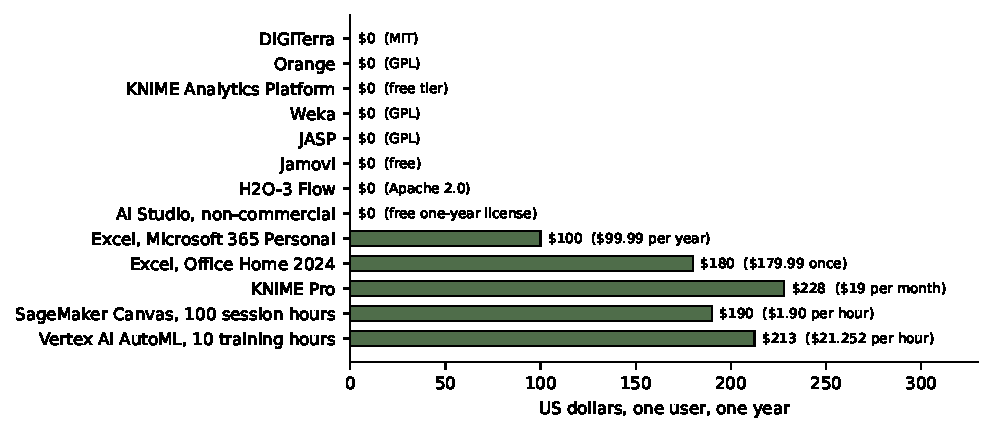
\includegraphics[width=0.85\textwidth]{fig_price_scenario}
\caption{Stated price under one scenario: one user, one year, about 100 hours of modeling. Desktop tools cost their license; SageMaker Canvas is charged at the session rate for 100 hours; Vertex AI at the training rate for 10 training hours (session time is not billed as such); KNIME Pro at twelve months. Azure Machine Learning, DataRobot and AI Studio's commercial tier carry no list price on the pages read and are not drawn. Excel is shown under both purchase forms. Source: \code{docs/price\_survey\_2026-09-25.txt}.}
\label{fig:price}
\end{figure}

The scenario in Figure~\ref{fig:price} is one reading of the stated prices, not a total cost of ownership. A cloud service's bill depends on the compute chosen, the data stored and the hours logged in, and the free tiers change; a desktop tool's cost is the machine the group already owns. The point the figure carries is narrower: for the workflow the product comparison describes, a fitted and documented model on one table, every desktop product in the table is available at no charge, and the cloud products bill from the first hour after their free tier.

\section{Accessibility claims}
\label{sec:access}

DiGiTerra's guided page is built to WCAG 2.2 AA: landmarks, a label for every control, live regions for errors and progress, focus that moves only where the user's own action opened the next step, and no meaning carried by color alone. A Chromium test runs axe-core under the WCAG A and AA rule sets with no serious violation allowed, reads a typed hyperparameter back from the fitted estimator, and walks the page by keyboard; \code{docs/ACCESSIBILITY.md} states what is checked and what is not claimed, and \code{docs/guided\_page\_aria\_transcript.txt} is the accessible-name transcript of the page. What is not claimed is a screen-reader session with a human user; the checks are automated.

Among the compared products, the feature survey found three kinds of statement. The cloud vendors publish conformance reports: AWS an ACR/VPAT covering Section 508 and WCAG for SageMaker, Microsoft ACRs for WCAG, Section 508 and EN 301 549, and Google a VPAT list that names Vertex AI Tabular Data. Two of the free desktop tools publish their own statements: jamovi's says the interface ``can be operated entirely from the keyboard and works with NVDA and JAWS'', and JASP's VPAT of August 2025 says ``JASP does not currently support screen readers''. Orange, KNIME, Weka, AI Studio and DataRobot state nothing on the pages read; H2O Flow documents keyboard shortcuts only. A statement is not a test, and this section records the statements.


\section{Operating notes for the EDX copy}
Before any release to EDX: run \code{MPLBACKEND=Agg python scripts/adversarial\_check.py --json docs/adversarial\_check\_<date>.json} and require 10 of 10; run the sweep and the round trip when the registry or the artifact code changes; rebuild the desktop bundle with \code{pyinstaller build/DiGiTerra.spec} and confirm that \code{Contents/Resources/examples} is present and that a model trains in the built app (the 2026-09-25 build, PyInstaller 6.22.3 on Python 3.13.1, exit 0, 402 MB, has not yet been launched). Keep the E1 folder unchanged as the reference set; a new differential run goes in a new folder with its own date. The Orange C2 attribution is the one open item and is closed by running \code{scripts/oracle.py} under Orange's bundled Python on an arm64 Mac.

\section{Sources}
\label{sec:sources}

Repository records, all at commit \code{4e49ba9} of \code{github.com/rowanterra/DiGiTerra}, branch \code{audit-fixes}:

\begin{itemize}
\item \code{docs/differential\_test\_E1/}: \code{PLAN.txt}, \code{PROTOCOL.txt}, \code{NOTEBOOK.txt}, \code{RESULTS.csv}, \code{RESULT\_2026-09-24.txt}, \code{RESULT\_2026-09-25.txt}, \code{data/}, \code{oracle\_outputs/}, \code{reference\_outputs/}, \code{digiterra\_outputs/}, \code{digiterra\_outputs\_pre\_fix\_0942e0c/}, \code{scripts/}.
\item \code{CHANGELOG.md}, section 0.1.0; \code{tests/unit/test\_review\_2026\_09\_24.py}; \code{tests/unit/test\_bundle.py}; \code{tests/unit/test\_decimal\_setting.py}; \code{scripts/adversarial\_check.py}; \code{docs/adversarial\_check\_2026-09-24.json}; \code{docs/adversarial\_check\_2026-09-25.json}.
\item \code{docs/every\_model\_sweep\_2026-09-24.json}; \code{docs/artifact\_roundtrip\_2026-09-24.json}; \code{python\_scripts/reporting/artifact\_allowlist.txt}.
\item \code{docs/competitor\_survey\_2026-09-24.txt}; \code{docs/price\_survey\_2026-09-25.txt}; \code{docs/ACCESSIBILITY.md}; \code{docs/guided\_page\_aria\_transcript.txt}; \code{templates/guided.html}.
\end{itemize}

Vendor pages, read on the date given; the quoted words in this document are from these pages:

\begin{itemize}
\item Amazon Web Services. SageMaker Canvas pricing. \url{https://aws.amazon.com/sagemaker/canvas/pricing/} (2026-09-25).
\item Microsoft. Azure Machine Learning pricing. \url{https://azure.microsoft.com/en-us/pricing/details/machine-learning/} (2026-09-25).
\item Google Cloud. Vertex AI pricing, section Tabular data. \url{https://cloud.google.com/vertex-ai/pricing} (2026-09-25).
\item KNIME. KNIME Hub pricing. \url{https://www.knime.com/knime-hub-pricing} (2026-09-25).
\item Altair. AI Studio Academic Hub. \url{https://web.altair.com/academic-hub-ai-studio} (2026-09-25); Altair Units license. \url{https://docs.rapidminer.com/2024.0/studio/installation/license/altair-units.html} (2026-09-25); Operator reference. \url{https://docs.rapidminer.com/latest/studio/operators/} (2026-09-25).
\item H2O.ai. Flow. \url{https://docs.h2o.ai/h2o/latest-stable/h2o-docs/flow.html} (2026-09-25).
\item jamovi. jamovi Cloud. \url{https://www.jamovi.org/cloud.html} (2026-09-25); Accessibility. \url{https://www.jamovi.org/accessibility.html} (2026-09-24).
\item JASP. Accessibility. \url{https://jasp-stats.org/accessibility/} (2026-09-24).
\item DataRobot. Pricing. \url{https://www.datarobot.com/pricing/} (2026-09-25).
\item Microsoft. Office Home 2024. \url{https://www.microsoft.com/en-us/microsoft-365/p/office-home-2024/cfq7ttc0pqvj} (2026-09-25); Compare all Microsoft 365 products. \url{https://www.microsoft.com/en-us/microsoft-365/buy/compare-all-microsoft-365-products} (2026-09-25).
\item Orange. License. \url{https://orangedatamining.com/license/} (2026-09-24).
\item Homebrew formulae API for the cask versions installed: knime 5.12.0, jasp 0.98.1.0, jamovi 2.7.37.0; Weka 3.8.7 from \url{https://sourceforge.net/projects/weka/} (2026-09-25).
\end{itemize}

Installed copies driven on 2026-09-25: Orange 3.39.0, Altair AI Studio 2026.0.1, KNIME Analytics Platform 5.12.0, Weka 3.8.7 (OpenJDK 21), JASP 0.98.1, jamovi 2.7.37, Microsoft Excel 16.03, all on macOS (Apple silicon); H2O-3 3.46.0.7 under Python 3.11 in a Linux container; DiGiTerra at \code{4e49ba9} in the same container.


\section*{Substitution list}
No term was replaced for review; the wording of the audit sections is the wording of the repository records.

\end{document}
